\documentclass{article}
\usepackage[a4paper, margin=1in]{geometry}
\usepackage[utf8]{inputenc}
\usepackage[T1]{fontenc}
\usepackage{lmodern}
\usepackage{amsmath, amssymb, graphicx, hyperref}
\usepackage{bookmark}
\graphicspath{{../figures/}}
\usepackage[framed,numbered]{matlab-prettifier}
\usepackage{xcolor}
\usepackage{listings}

\geometry{a4paper, margin=1in}

% MATLAB code style
\lstset{
  style      = Matlab-editor,
  basicstyle = \mlttfamily,
  breaklines = true
}

\title{\textbf{Practical - 1}}
\author{}
\date{October 3, 2026}

\pagenumbering{gobble}

\begin{document}
\maketitle
\thispagestyle{empty}

\noindent
\textbf{\large{Aim:}} To solve first order ordinary differential equation and plot its solution.

\vspace{1em}
\noindent
\textbf{\large{MATLAB Code:}}

\begin{lstlisting}
clc; clear all; close all;

syms y(x)

eqn =  diff(y,1) + 2*y - 12*sin(4*x) == 0;
init = y(0) == 10;

ysol = dsolve(eqn, init);
disp(ysol)

fplot(ysol, [0,8]);
axis([0 8 -3 7]);
grid on;
title('Plotting of first order ODE');
xlabel('x-axis')
ylabel('y-axis')
\end{lstlisting}

\vspace{1em}
\noindent
\textbf{\large{Output:}}

\vspace{0.5em}

\begin{flushleft}
$\frac{62\,{\mathrm{e}}^{-2\,x} }{5}-\frac{6\,\sqrt{5}\,\cos \left(4\,x+\mathrm{atan}\left(\frac{1}{2}\right)\right)}{5}$
\end{flushleft}

\vspace{0.5em}

\begin{figure}[htbp]
    \centering
    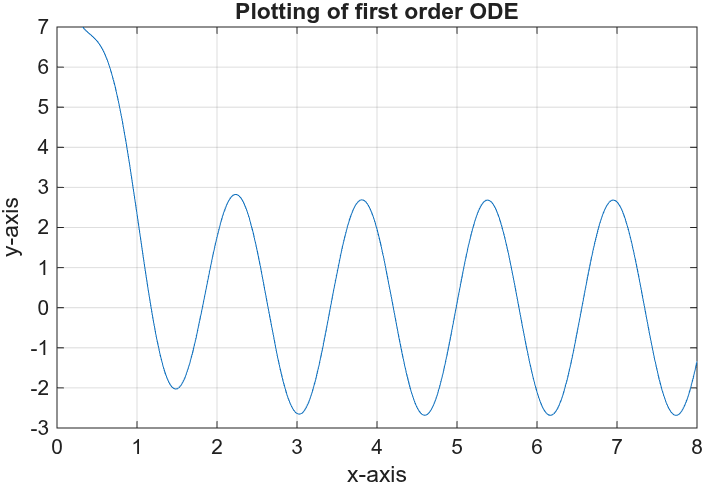
\includegraphics[width=0.6\textwidth]{Figure1.png}
\end{figure}


\end{document}
